

\subsubsection{Tavola dei Volumi}

% Note per noi:
% - Giorni in un anno: 280
% - Settimane in un anno: 46
Abbiamo stimato che la base di dati ha un ciclo di vita di 5 anni.


% Il gioco in questione \'{e} in fase di progettazione, quindi i volumi delle entit\'{a} e delle relazioni sono stati individuati su una stima di mercato,che prevede il raggiungimento dei valori proposti entro i primi tre mesi di gioco. Solitamente in questo periodo si ha il boom di iscrizioni ad un gioco online, che poi vanno a diminuire di molto nel tempo cos\`{\i}come l'attività dei giocatori. I dati indicati con (**) variano velocemente nel tempo e sono pertanto molto indicativi.

\noindent\makebox[\textwidth]{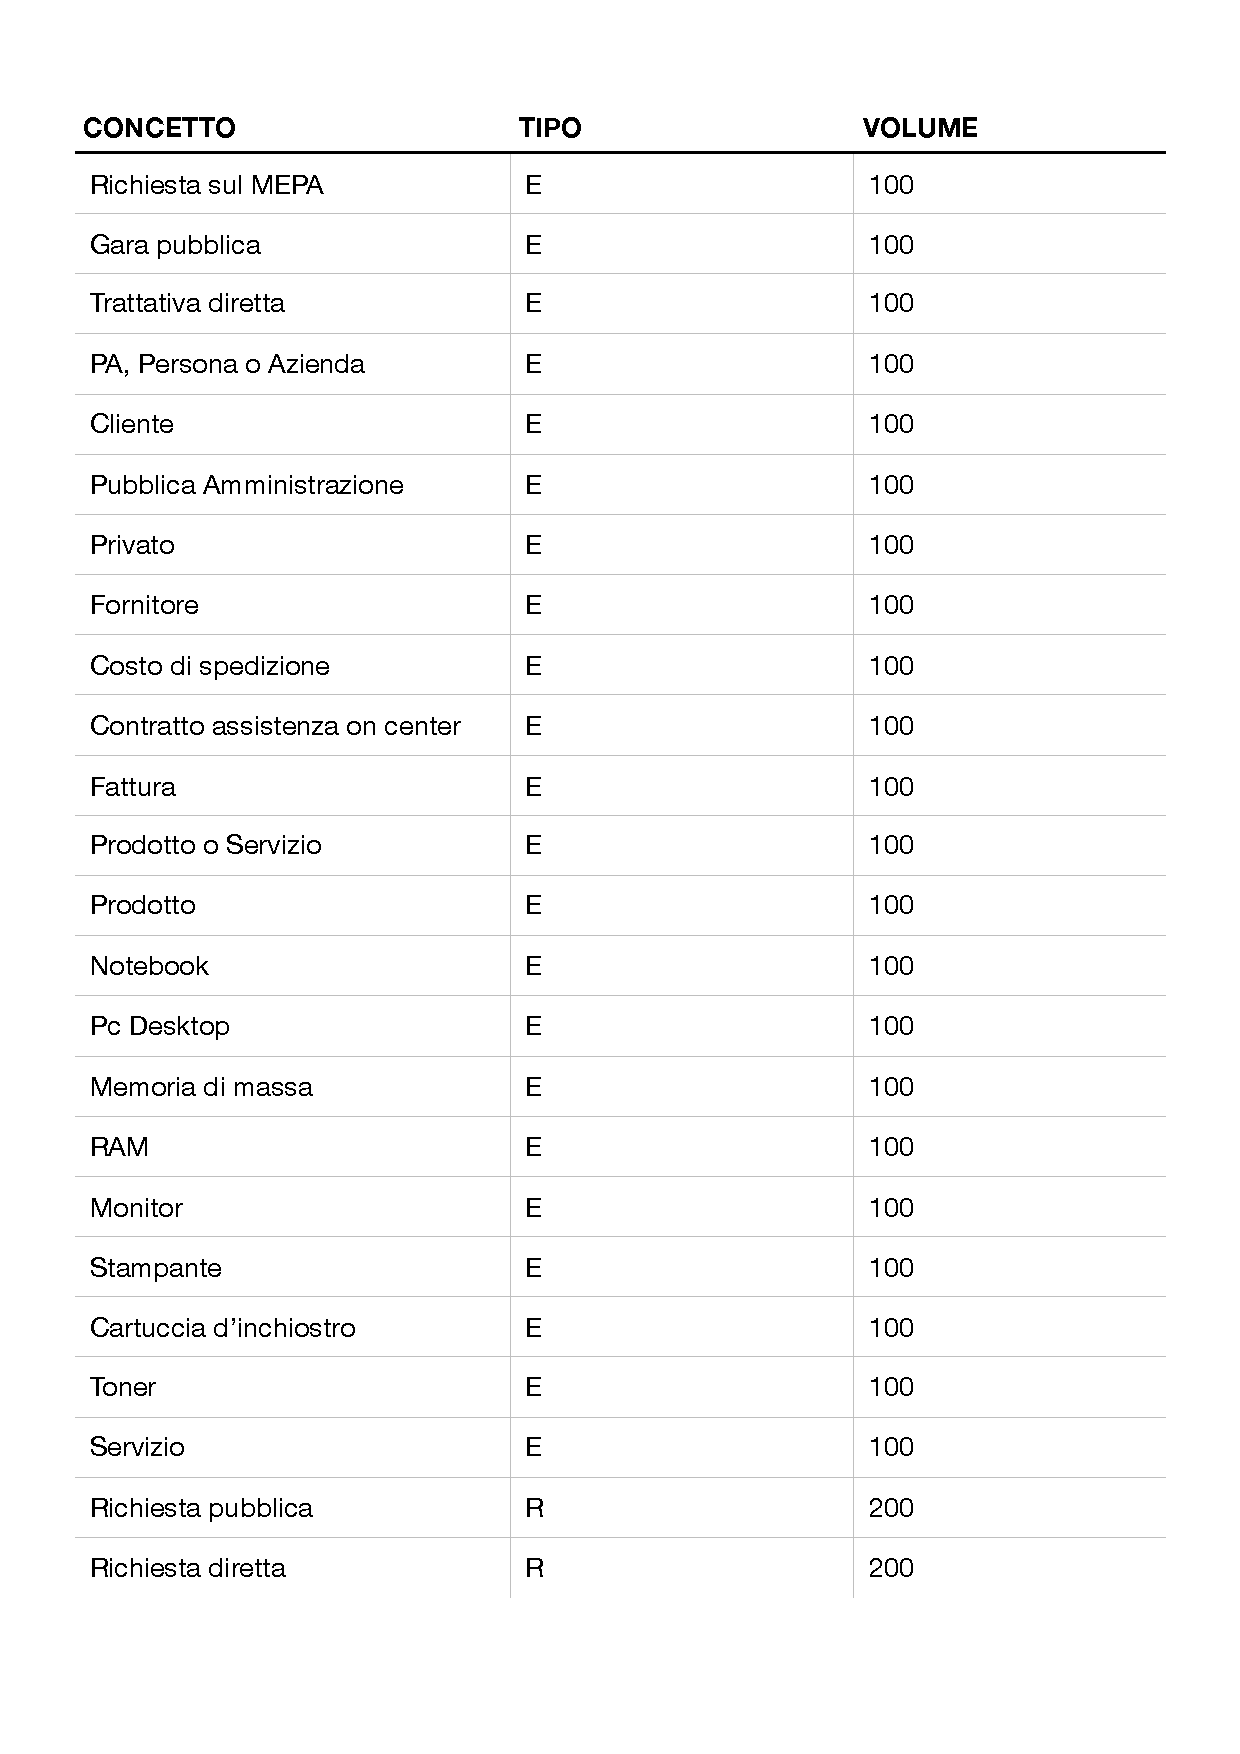
\includegraphics[page=1, width=\textwidth+1.5cm]{./pdf/tavola_volumi.pdf}}
\noindent\makebox[\textwidth]{\includegraphics[page=2, width=\textwidth+1.5cm]{./pdf/tavola_volumi.pdf}}


\subsubsection{Tavola delle Operazioni}

\noindent\makebox[\textwidth]{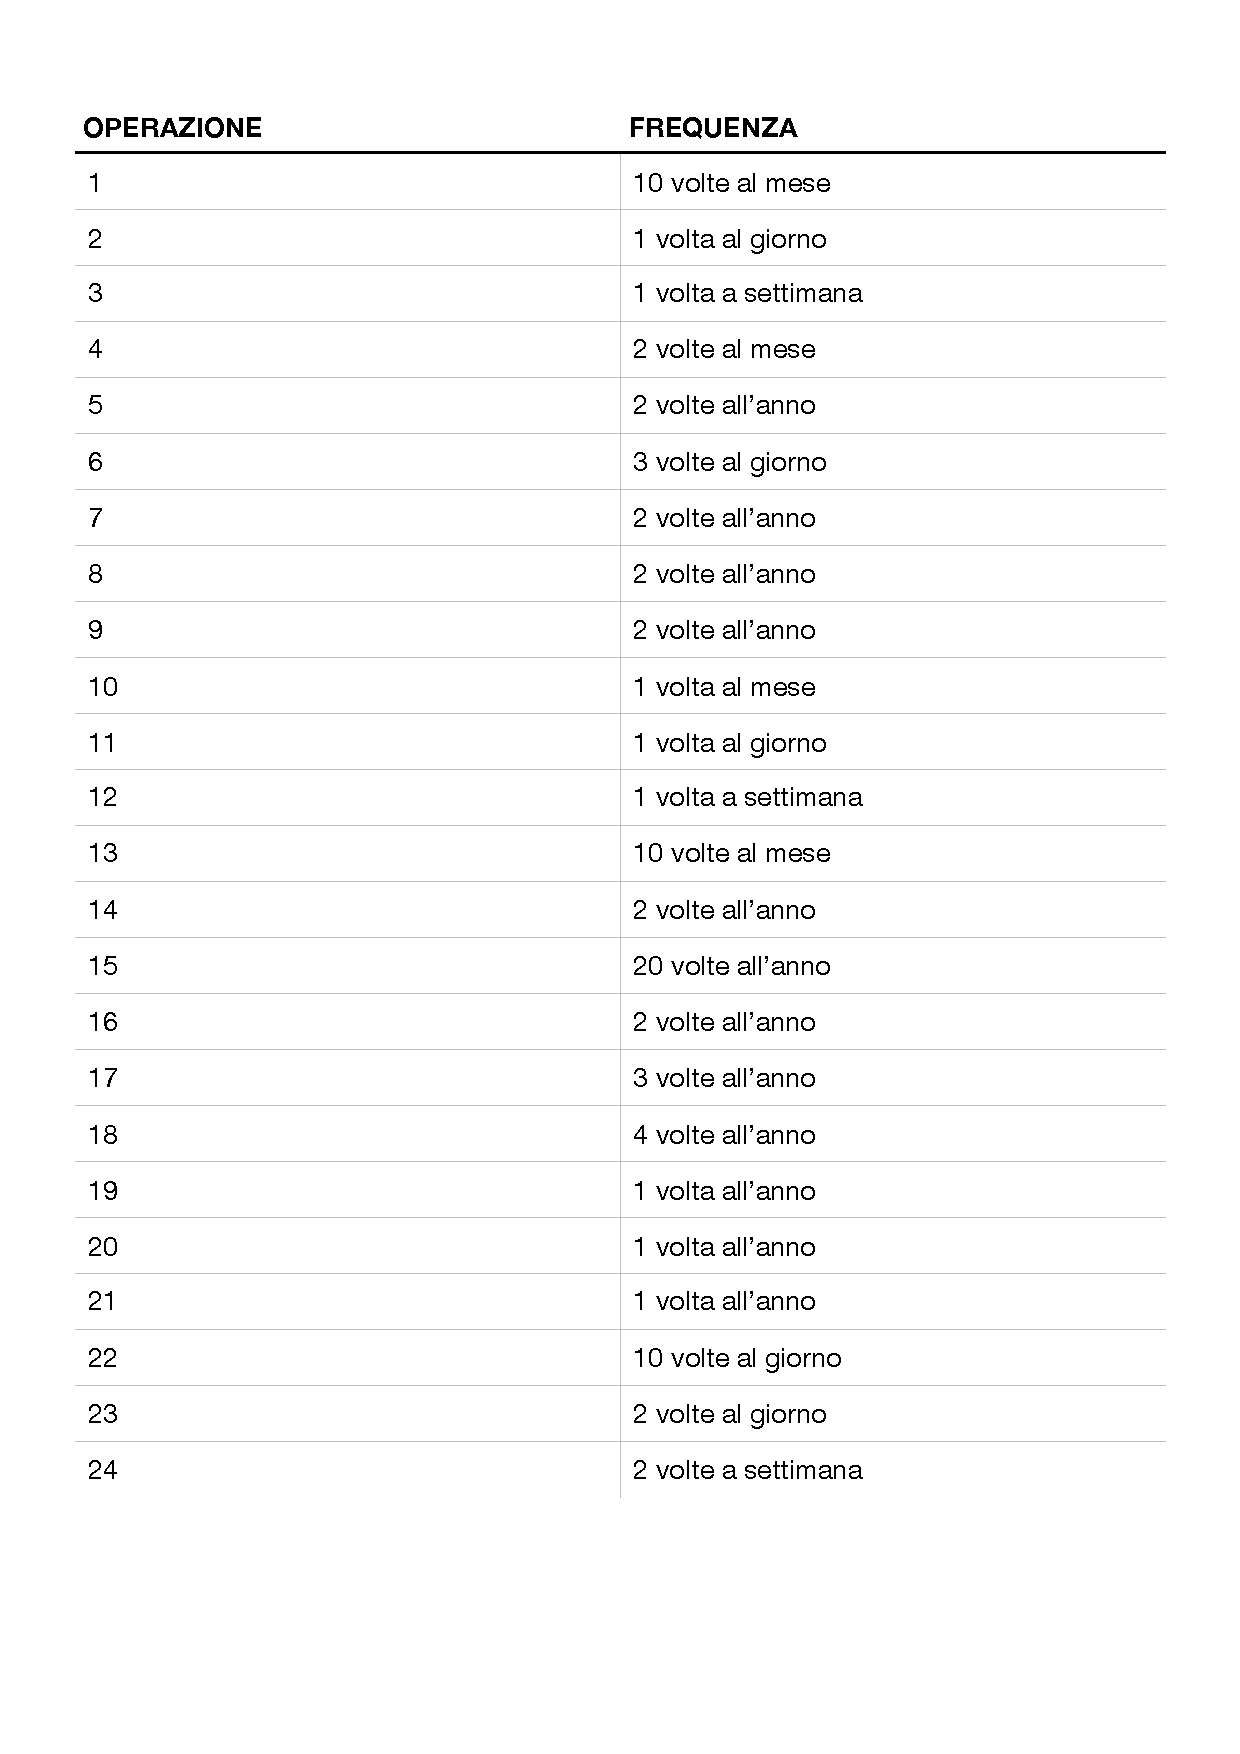
\includegraphics[page=1, width=\textwidth+1.5cm]{./pdf/tavola_operazioni.pdf}}
\newpage
\noindent\makebox[\textwidth]{\includegraphics[page=2, width=\textwidth+1.5cm]{./pdf/tavola_operazioni.pdf}}
